\documentclass[a4paper]{article}
\usepackage[utf8]{inputenc} 
\usepackage[danish]{babel} 

\usepackage{amsmath}
\usepackage{amsfonts}
\usepackage{amssymb}
\usepackage{ulem}
\usepackage{verbatim}
\usepackage{graphicx}

\newcommand{\setR}{\mathbb{R}} 
\newcommand{\setF}{\mathbb{F}} 
\newcommand{\setN}{\mathbb{N}} 
\newcommand{\pder}[2][]{\frac{\partial#1}{\partial#2}}


\title{Assignment 49, the Wave Equation}
\author{Beate, Sarah og Freja}
\begin{document}
\maketitle

\section*{Part (A)}
$$
c^2* \pder{u}{x}(x,t)= \pder{u}{t^2}(x,t), \quad x \in (o,l), \quad t>0 \quad\textbf{(1)}
$$
\\
$$
\pder{u}{x} \approx \frac{u(x_{i+1},t_j)-2u(x_i,t_j)+u(x_{i-1},t_j)}{h^2} \quad \textbf{(2)}
$$
$$
\pder{u}{t} \approx \frac{u(x_i,t_{j+1})-2u(x_i,t_j)+u(x_i,t_{j-1})}{k^2} \quad \textbf{(3)}
$$
\\
\textit{Isolating:} \\
We are aproximating \textbf{(2)} and \textbf{(3)} by insterting them in \textbf{(1)}.

$$
(\frac{k^2}{1})*\frac{c^2(u(x_{i+1},t_j)-2u(x_i,t_j)+u(x_{i-1},t_j))}{h^2}=\frac{u(x_i,t_{j+1})-2u(x_i,t_j)+u(x_i,t_{j-1})}{k^2}*(\frac{k^2}{1}) \rightarrow
$$
$$
\frac{(u(x_{i+1},t_j)-2u(x_i,t_j)+u(x_{i-1},t_j))c^2k^2}{h^2}=u(x_i,t_{j+1})-2u(x_i,t_j)+u(x_i,t_{j-1}) \rightarrow 
$$
$$
u(x_i,t_{j+1})=\frac{(u(x_{i+1},t_j)-2u(x_i,t_j)+u(x_{i-1}),t_j))c^2k^2}{h^2}+2u(x_i,t_j)-u(x_i,t_{j-1}) \quad \textbf{(4)}
$$
\\
\textit{Grouping:} \\
Can see that we have two of the same variables, $2u(x_i,t_j)$, which we'll group together, based on our derived equation  \textbf{(4)},
$$u(x_i,t_{j+1})=\frac{(u(x_{i+1},t_j)-2u(x_i,t_j)+u(x_{i-1},t_j))c^2k^2}{h^2}+2u(x_i,t_j)-u(x_i,t_{j-1})$$
\\
To simplifiy things, will we make a constant $\lambda=\frac{c^2k^3}{h^2}$ and we get
$$
u(x_i,t_{j+1})=\lambda(u(x_{i+1},t_j)-2u(x_i,t_j)+u(x_{i-1},t_j))+2u(x_i,t_j)-u(x_i,t_{j-1}) \rightarrow
$$
$$
u(x_i,t_{j+1})=\lambda u(x_{i+1},t_j)-2\lambda u(x_i,t_j)+ \lambda u(x_{i-1},t_j)+2u(x_i,t_j)-u(x_i,t_{j-1}) \rightarrow
$$
\\
The final result,
$$
\uuline{u(x_i,t_{j+1})=\lambda u(x_{i+1},t_j)+\lambda   u(x_{i-1},t_j)-u(x_i,t_{j-1})-2\lambda u(x_i,t_j)+2u(x_i,t_j)}
$$
\\
\section*{Part (B)}
\begin{figure} [h]
\centering 
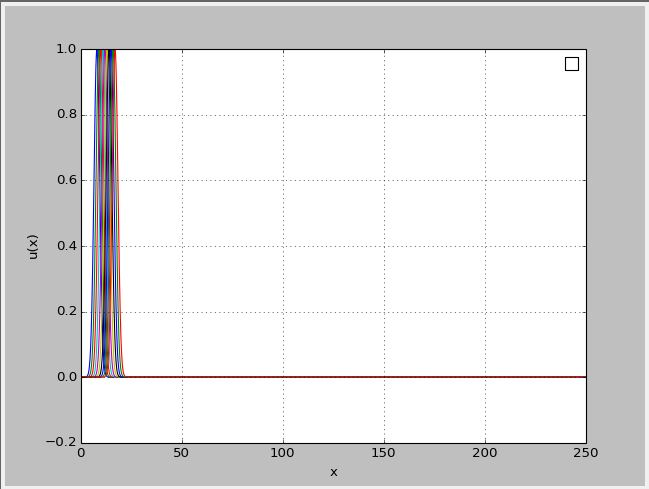
\includegraphics[width=90mm]{1}
\caption{u(x,t) as a function of x with a constant time, t.}
\label{fig:1}
\end{figure}

\section*{Part (C)}
When $c=1$, $l=250$ and the wave have travel around the stadium, then we are at the end of our grid. To have the exact time requires a 3D graph which we attempted but failed to program. 
\begin{figure} [h]
\centering
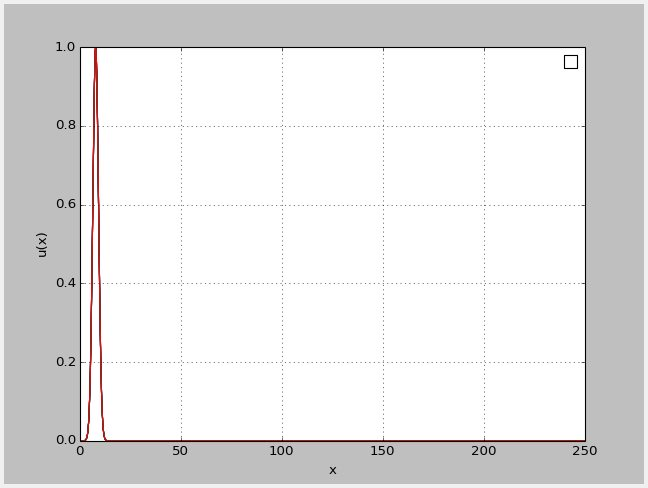
\includegraphics[width=90mm]{2}
\caption{When t=0.}
\label{fig:2}
\end{figure}
\begin{figure} [h]
\centering
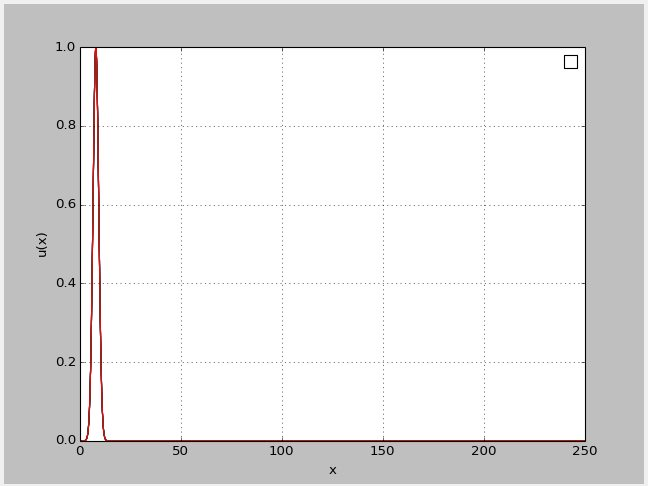
\includegraphics[width=90mm]{3}
\caption{When t=k.}
\label{fig:3}
\end{figure}
\begin{figure} [h]
\centering
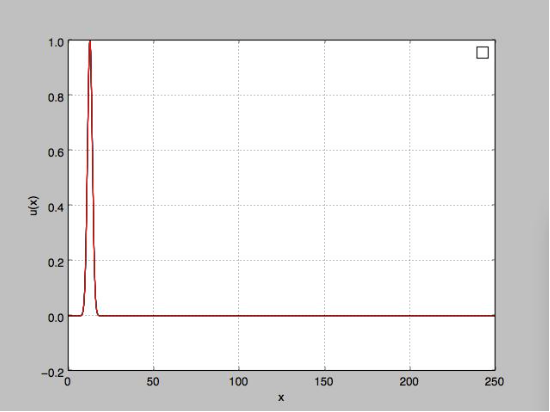
\includegraphics[width=90mm]{4}
\caption{When the wave have reached half-way arround the stadion, thus the wave have reached half of our choosen value grid(50). Plotting index u[:,50].}
\label{fig:4}
\end{figure}
\begin{figure} [h]
\centering
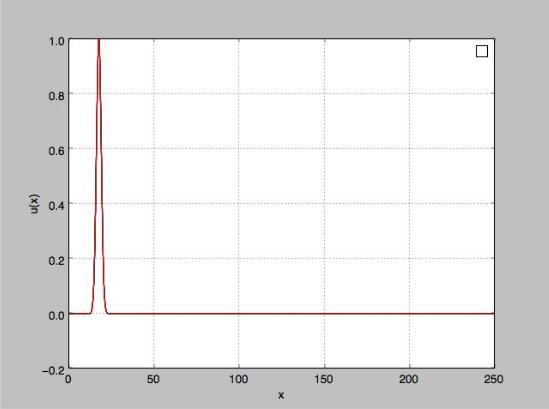
\includegraphics[width=90mm]{5}
\caption{The wave have reached the end of the stadion. The wave have reached the end of the grid(99), which we have indexed because when the wave hits the 100 mark the programme bounces of the grid.}
\label{fig:5}
\end{figure}
\begin{figure} [h]
\centering
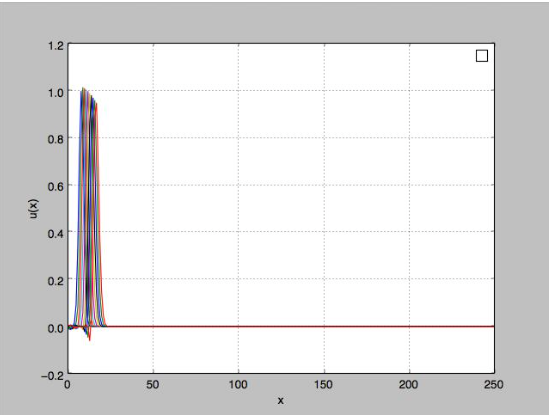
\includegraphics[width=90mm]{6}
\caption{When step size, h, is changed. In this case h=1, resulting in out of bounce when t=0.}
\label{fig:6}
\end{figure}
\begin{figure} [h]
\centering
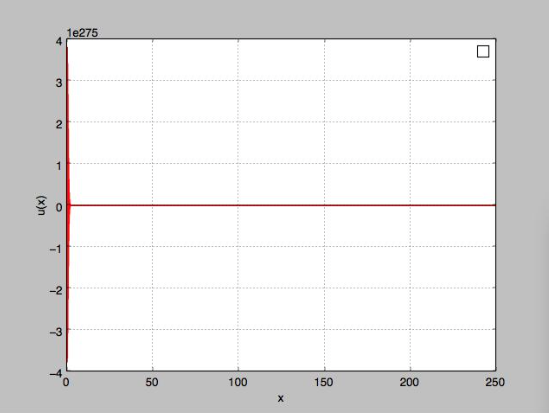
\includegraphics[width=90mm]{7}
\caption{When step size, k, is changed. In this case k=2, resulting in out of bounce when t=k.}
\label{fig:7}
\end{figure}

\begin{figure}
\centering
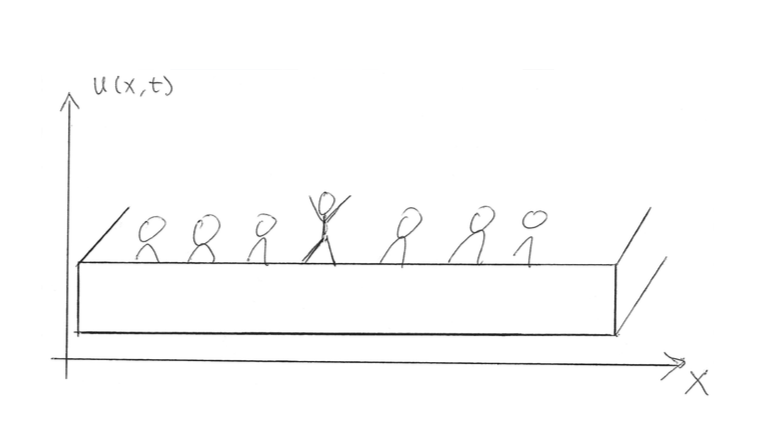
\includegraphics[width=120mm]{TheWave}
\caption{Audience at a stadion making a "wave," have a nice weekend.}
\label{fig:The Wave}
\end{figure}

\end{document}